
\chapter{Triangulierte Objekte}

Komplexe Objekte wie der Stanford Bunny bestehen aus einem Polygonnetz. Die einfachste Form des Polygons ist das Dreieck und die so zusammengesetzten Objekte sind triangulierte Objekte.
Im Abschn.~\ref{sec:dreieck} wurde bereits gezeigt wie man den Schnittest und die Berechnung der Normalen für Dreiecke durchführt.
Die naive Erweiterung um triangulierte Objekte beim "`Raytracing"' verwenden zu können, besteht darin, für jedes einzelne Dreieck im Dreiecksnetz eben diese Schritte durchzuführen. Wenn das triangulierte Objekt nur aus wenigen Dreiecken besteht, ist diese Vorgehensweise noch durchführbar. Der Stanford Buddha besteht jedoch aus über einer Million Dreiecke, wovon jedes mit jedem Strahl getestet werden müsste. In Kapitel~\ref{ch:beschleunigung} werden deshalb Beschleunigungsstrukturen vorgestellt, um die Anzahl durchgeführter Schnitttests zu reduzieren.

\section{Das OBJ-Format}

Zur Repräsentation eines Dreiecksnetzes existieren Dateiformate wie das OBJ-Format von Wavefront~\cite{reddy2015obj}. Das OBJ-Format erlaubt eine kompakte Darstellung des Polygonnetzes, indem alle vorkommenden Punkte aufgelistet werden und die jeweiligen Polygone durch Referenzierung der Punktindices definiert werden. Dadurch werden Punkte, die von mehreren Polygonen verwendet werden, nicht mehrmals gespeichert.

Das nun folgende Beispiel zeigt die Definition eines in der xy-Achse liegenden Quadrats. Es ist im Ursprung zentriert, hat eine Kantenlänge von 2 und ist aus zwei Dreiecken zusammengesetzt.

\begin{verbatim}
# Definition eines Quadrats im OBJ Format

v  -1.0   1.0  0.0
v  -1.0  -1.0  0.0
v   1.0   1.0  0.0
v   1.0  -1.0  0.0
# 4 Punkte

vn 0.0000 -0.0000 1.0000
# 1 Normale

f 1//1 2//1 3//1     # Punktindex/Texturkoordinate/Normalenindex
f 4//1 3//1 2//1     # Punktindex/Texturkoordinate/Normalenindex
# 2 Dreiecksfächen
\end{verbatim}

Die OBJ-Datei wird von oben nach unten abgearbeitet. Kommentare werden durch \texttt{\#} gekennzeichnet.
Definitionen werden durch Bezeichner eingeleitet und erhalten einen impliziten Index beginnend mit 1.
Als erstes werden Punkte definiert, eingeleitet durch den Bezeichner \texttt{v}. Die nachfolgenden Zahlen stehen für die x, y und z-Komponente eines Punktes im dreidimensionalem Raum. Der erste definierte Punkt erhält den Index 1. Für folgende Punkte wird der Index jeweils inkrementiert.
Als nächstes folgt die Definition von Punktnormalen, gekennzeichnet durch den Bezeichner \texttt{vn}. Die drei nachfolgenden Zahlen entsprechen wieder den einzelnen Komponenten. Die Angabe von Punktnormalen ist optional. 
Sollten keine Punktnormalen definiert sein, wird für jedes Dreieck eine Dreiecksnormale berechnet, wie in Abschn.~\ref{sec:dreieck} gezeigt.

 Zuletzt folgt die Definition der Polygone, in diesem Fall Dreiecke, durch \texttt{f}. Die nachfolgenden Spalten folgen dem Schema \texttt{Punktindex/Texturkoordinatenindex/Normalenindex}. Im angegebenen Beispiel wird das erste Dreieck somit aus dem ersten, zweiten und dritten Punkt erzeugt. Texturkoordinaten werden zur Einfachheit im Beispiel ausgelassen. In Kapitel~\ref{ch:texturierung} wird aber noch konkret gezeigt, wie Texturkoordinaten aussehen. Zuletzt wird jedem Dreieckspunkt eine optionale Punktnormale durch \texttt{Normalenindex} zugewiesen. Falls keine Punktnormalen in der OBJ-Datei enthalten sind, können diese nachträglich berechnet werden wie der nachfolgende Abschnitt zeigt.
 
 Das vorgestellte (Minimal-) Beispiel ist so einfach, dass es noch ohne Probleme händisch erstellt werden kann. Für sehr komplexe Objekte, die z.B. aus mehreren zehntausend Polygonen bestehen und mehrere Texturen verwenden, benötigt man eine 3D-Modellierungssoftware zur Erstellung einer solchen Datei, weshalb "`3ds Max"' von "`Autodesk"' zur Erstellung und Bearbeitung von 3D-Modellen benutzt wird. Zum Laden von 3D-Modellen kommt neben dem selbstgeschriebenen OBJ-Parser noch die quelloffene Bibliothek "`Assimp"' zum Einsatz, die eine Vielzahl an Formaten für 3D-Modelle unterstützt.


\section{Facettierte und glatte Schattierung} \label{sec:facetierte_und_glatte_schattierung}

Abb.~\ref{fig:konstante_schattierung} zeigt den "`Stanford Bunny"' in facettierter Schattierung. Diese Art der Schattierung erhält man, wenn man pro Dreieck eine einzige Dreiecksnormale verwendet. Die einzelnen Dreiecke sind dann gut erkennbar, da sich die Farbe innerhalb eines Dreiecks nicht großartig verändert. Dies hat folgenden Grund: Unabhängig von der Lage des Schnittpunkts wird immer die gleiche Dreiecksnormale verwendet. Die einzige, für die Schattierung relevante Komponente, die sich mit der Lage des Schnittpunkts ändert, ist der Einfallswinkel der Lichtstrahlen. Bei entsprechend kleinen Dreiecken ändert sich der Einfallswinkel des Lichtstrahls nur geringfügig, wodurch der Eindruck entsteht, dass das Dreieck einfarbig ist.
Um den "`Bunny"' so zu schattieren, wurde eine OBJ-Datei geladen, die lediglich Polygone sowie entsprechende Punkte enthält. Da im OBJ-Format die Polygone mit einem Umlaufsinn gegen den Uhrzeigersinn definiert werden, kann eine Dreiecksnormale direkt nach der Vorgehensweise aus Abschn.~\ref{sec:dreieck} berechnet werden.

Im Gegensatz dazu zeigt Abb.~\ref{fig:glatte_schattierung} wie eine glatte Schattierung erzielt werden kann, indem sich die Normale abhängig vom Schnittpunkt ändert. Dies geschieht durch Interpolation der Punktnormalen. Seien \( \boldsymbol{n_0}, \boldsymbol{n_1} \text{ und } \boldsymbol{n_2} \) die Punktnormalen, die den Dreieckspunkten (z.B. durch die OBJ-Datei) zugewiesen sind. Bei Durchführung des Dreieckschnitttests erhält man die baryzentrischen Koordinaten \( \beta \text{ und } \gamma \), die die Position des Schnittpunkts innerhalb des Dreiecks widerspiegeln (siehe Abschn.\ref{sec:dreieck}). Diese Koordinaten werden nun zur Berechnung der Normalen am Schnittpunkt \( \boldsymbol{n_{\boldsymbol{r}}} \) benutzt:

\begin{equation*}
    \boldsymbol{n_{\boldsymbol{r}}} = (1 - \beta - \gamma) \cdot \boldsymbol{n_0} + \beta \cdot \boldsymbol{n_1} + \gamma \cdot \boldsymbol{n_2}
\end{equation*}

Wie bereits erwähnt, ist die Angabe der Punktnormalen optional und so ist es möglich, dass keine in der OBJ-Datei vorhanden sind. Es gibt jedoch die Möglichkeit, diese nachträglich zu berechnen. Falls keine Punktnormalen vorhanden sind, wird für jedes Dreieck eine Dreicksnormale berechnet. Möchte man nun für einen bestimmten Punkt die Punktnormale berechnen, so iteriert man über alle angrenzenden Dreiecke, die diesen Punkt verwenden, und summiert deren Dreiecksnormalen auf. Die resultierende Normale ist jedoch kein Einheitsvektor mehr und muss normalisiert werden, falls diese Eigenschaft gefordert ist.


%\begin{algorithm}[H]
%    \caption{Berechne Punktnormale für Dreickspunkt \( \boldsymbol{p_0} \)}
%    \label{alg:punktnormale}
%    \begin{algorithmic}[1]
%        \State \( \vv{n}_{res} \gets \vv{0} \) 
%        \For {each \( \text{Polygon } poly \in polygon\_enthalt\_p_0 \)}
%        \State \( \vv{n}_{res} \gets \vv{n}_{res} + dreicksnormale\_von(poly) \)
%        \EndFor
%        \State \( \vv{n}_{res} \gets \vv{n}_{res} \cdot |\vv{n}_{res}|^{-1} \)
%    \end{algorithmic}
%\end{algorithm}
%\todo{Algorithum muss definitiv formal besser aufgeschrieben werden.}
%



\begin{minipage}[t]{0.48\textwidth}
    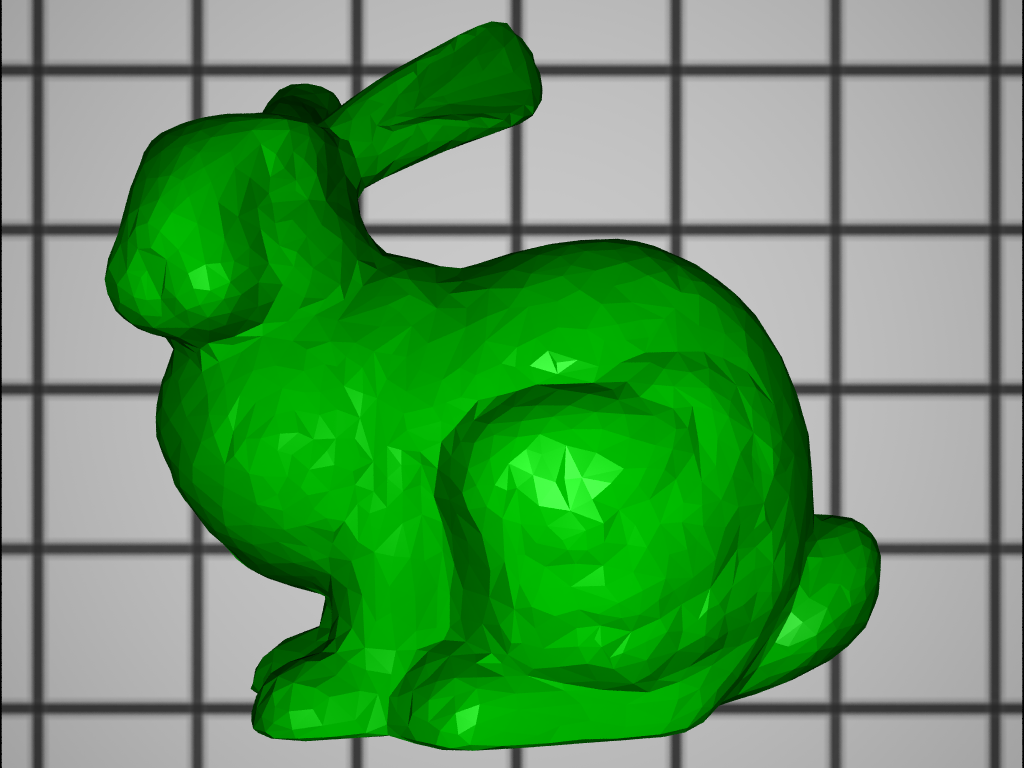
\includegraphics[width=\textwidth]{./img/triangulierte_objekte/konstante_schattierung.png}
    \captionof{figure}{Verwendung nur einer Normalen pro Dreieck führt zu facettierter Schattierung}
    \label{fig:konstante_schattierung}
\end{minipage}
\begin{minipage}[t]{0.48\textwidth}
    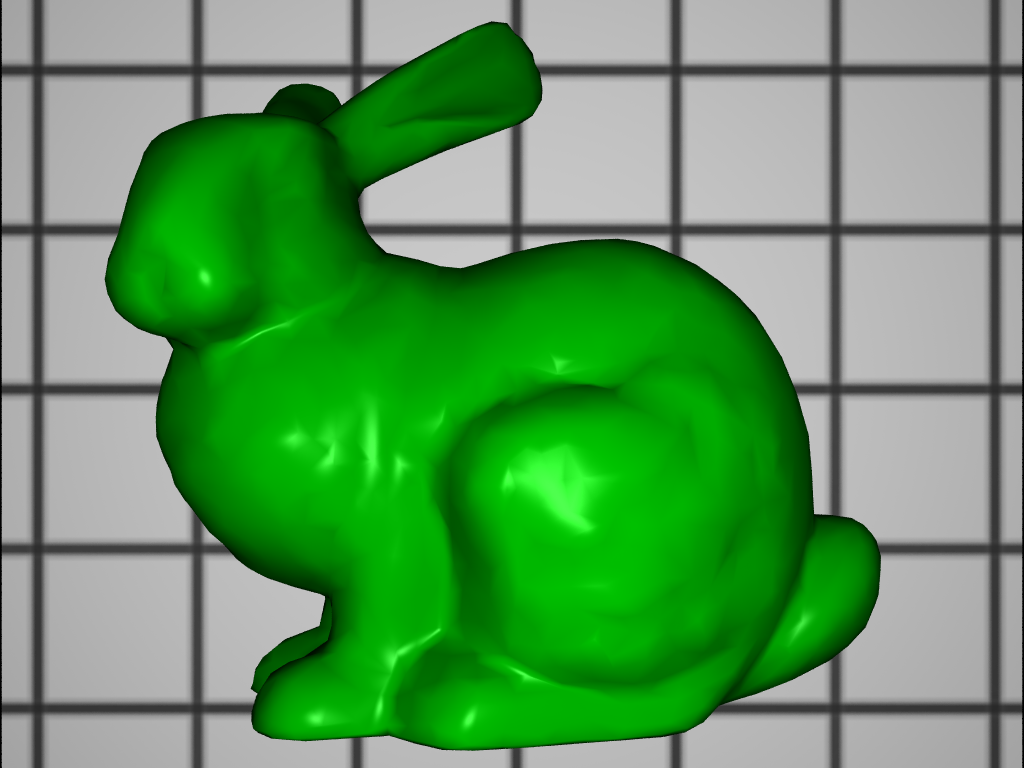
\includegraphics[width=\textwidth]{./img/triangulierte_objekte/glatte_schattierung.png}
    \captionof{figure}{Einbeziehung und Mittelwertbildung benachbarter Dreiecksnormalen sorgt für glattere Schattierung}
    \label{fig:glatte_schattierung}
\end{minipage}









\section{Instanziierung}

Durch Instanziierung kann ein einzelnes Polygonnetz für mehrere Objekte verwendet werden. Programmiertechnisch erzeugt man dazu eine Klasse, die eine Referenz auf das Polygonnetz enthält. Des weiteren speichert die Klasse eine Transformationsmatrix und deren Inverse, sowie Oberflächeneigenschaften in Form eines Materials. Mit dieser Ausstattung ist es möglich, zu prüfende Strahlen zu transformieren und den transformierten Strahl mit dem Polygonnetz zu testen. Dadurch lässt sich ein möglicher Schnittpunkt ermitteln. Die dabei erhaltene Normale wird entsprechend transformiert und zur Berechnung der Schattierung, durch das ebenfalls gespeicherte Material, verwendet. So lässt sich auf speicherplatzsparende Art ein und dasselbe Polygonnetz mit unterschiedlichen Transformationen und Schattierungen darstellen. Zudem wird die Laufzeit verkürzt, da das Polygonnetz nicht mehrmals geladen werden muss. Noch schwerer ins Gewicht fällt das Erzeugen einer Beschleunigungsstruktur, was dadurch ebenfalls reduziert wird (s. Unterabschnitt~\ref{subs:geschwindigkeitsmessung} ).
